\documentclass[12pt]{article}
\usepackage[margin=1in]{geometry}
\usepackage[all]{xy}


\usepackage{amsmath,amsthm,amssymb,color,latexsym}
\usepackage{geometry}        
\geometry{letterpaper}    
\usepackage{graphicx}
\usepackage[shortlabels]{enumitem}
\usepackage{import}
\usepackage{xifthen}
\usepackage{pdfpages}
\usepackage{transparent}
\newcommand{\incfig}[1]{%
    \def\svgwidth{\columnwidth}
    \import{./Figures/}{#1.pdf_tex}
}


\newtheorem{problem}{Problem}

\newenvironment{solution}[1][\it{Solution}]{\textbf{#1. } }{$\square$}


\begin{document}
\noindent TAM 445 Spring 2024\hfill Problem Set \#2\\
Jerich Lee. (02/8)

\hrulefill


\noindent In the following problems, let \(e_i \quad(i=1, 2, 3)\) denote three orthonormal basis vectors for a Euclidean vector space \(V\) equipped with the standard inner product \(u \cdot v = u_i v_i\) .

\begin{problem}
    Show that the set of nine tensors \(\{e_i \otimes e_j: i,j=1,2,3\}\) forms a basis for the real vector space of second-order tensors.
\end{problem}

If \(e_i\) and \(e_j\) represents three orthonormal basis vectors each \(\in V\) , then this implies that there exists \(f_i\) and \(g_i\) \(\in V^{\prime} \) such that

\[
    f_i(e_j) = \begin{cases}
        1,  &\text{ if } i=j ;\\
        0, &\text{ if } i \neq j ;\\
    \end{cases} = \delta_{ij} 
    \quad \text{and} \quad
    g_j(e_i) = \begin{cases}
        1,  &\text{ if } j=k ;\\
        0, &\text{ if } j \neq k ;\\
    \end{cases} = \delta_{ji} 
\]

Suppose that there exists a list of scalars \(\left\{ a_{j,k} \right\} \) such that

\[
    a_{i,j}(e_{i} \otimes e_j)=0 \tag{1} 
\]

We can also state the following:

\[
    (e_i \otimes e_j)(f_M \otimes g_N)= \begin{cases}
        1,  &\text{ if } i=M ;\\
        0, &\text{ if } j = N ;\\
    \end{cases} \tag{2}
\]

Multiplying both sides of Equation 2 by 1, we get the following:

\begin{align*}
    a_{i,j}(e_{i} \otimes e_j)(f_M \otimes g_N)&=0(f_M \otimes g_N) \\
    a_{M,N} &= 0
\end{align*}

This shows that the scalar coefficient \(a_{M,N}\) is equal to \(0\), which implies that the original list of tensors \(e_i \otimes  e_j\) is linearly independent, which implies that this set is also a basis.

\begin{problem}
        a) Show that an example that the dyadic product is not commutative. In other words,
        \[
        \textbf{\textit{u}} \otimes \textbf{\textit{v}}   = \textbf{\textit{v}} \otimes  \textbf{\textit{u}}   \quad \forall \textbf{\textit{u}} , \textbf{\textit{v}}  \in V \tag{1}
        \]
        is \textit{not} true.
    \end{problem}
        We can provide a counterexample to prove this statement. Suppose that the dyadic product is commutative, and we define vectors 
        \[ \underline{\textbf{\textit{v}}} = 
            \begin{bmatrix}
                 1 \\
                 2 \\
                 3 \\
            \end{bmatrix},\underline{\textbf{\textit{u}}} = 
            \begin{bmatrix}
                 4 \\
                 5 \\
                 6 \\
            \end{bmatrix},
            \underline{\textbf{\textit{w}}} =
            \begin{bmatrix}
                 7 \\
                 8 \\
                 9 \\
            \end{bmatrix}
        \]

        The following is the definition of a tensor product:
\[
    (\underline{\textbf{\textit{u}} } \otimes \underline{\textbf{\textit{v}} } )\underline{\textbf{\textit{w}} } = (\underline{\textbf{\textit{v}} } \cdot \underline{\textbf{\textit{w}} } )\underline{\textbf{\textit{u}} } 
\]

\[
    (\underline{\textbf{\textit{u}} } \otimes \underline{\textbf{\textit{v}} } )\underline{\textbf{\textit{w}} } = (\underline{\textbf{\textit{v}} } \cdot \underline{\textbf{\textit{w}} } )\underline{\textbf{\textit{u}} } = \begin{bmatrix}
        1 \\
        2 \\
        3 \\
   \end{bmatrix}\cdot\begin{bmatrix}
    7 \\
    8 \\
    9 \\
\end{bmatrix} 
\]
$$
(\underline{\textbf{\textit{u}} } \otimes \underline{\textbf{\textit{v}} } )\underline{\textbf{\textit{w}} } = (\underline{\textbf{\textit{v}} } \cdot \underline{\textbf{\textit{w}} } )\underline{\textbf{\textit{u}} } = \left(\begin{bmatrix}
1 \\
2 \\
3
\end{bmatrix}\cdot \begin{bmatrix}
7 \\
8 \\
9
\end{bmatrix}\right)\begin{bmatrix}
4 \\
5 \\
6
\end{bmatrix}=\begin{bmatrix}
200 \\
250 \\
300
\end{bmatrix}
$$

\[
    (\underline{\textbf{\textit{v}} }\otimes \underline{\textbf{\textit{u}} })\underline{\textbf{\textit{w}} }=(\underline{\textbf{\textit{u}} }\cdot \underline{\textbf{\textit{w}} })\underline{\textbf{\textit{v}} }=\left(\begin{bmatrix}
        4 \\
        5 \\
        6
        \end{bmatrix}\cdot \begin{bmatrix}
        7 \\
        8 \\
        9
        \end{bmatrix}\right)\begin{bmatrix}
        1 \\
        2 \\
        3
        \end{bmatrix}=\begin{bmatrix}
        122 \\
        244 \\
        366
        \end{bmatrix}
\]

\[\begin{bmatrix}
    200 \\
    250 \\
    300
    \end{bmatrix} 
\neq     \begin{bmatrix}
        122 \\
        244 \\
        366
        \end{bmatrix}
\]
\vspace*{1cm}
Therefore, the tensor product is not commutative. 

        \begin{problem}
            b) Consider a vector \(\textbf{n}\in V\)   with \(\lVert n\rVert =1 \). Such vectors are referred to as \(\textit{unit vectors}\). Examine how the tensor 
        \[
            \textbf{\textit{I}}  - \textbf{\textit{n}}  \otimes \textbf{\textit{n}}  \tag{2} 
        \]  
        
        operates on vectors. Describe in words, the geometric significance of the above tensor.
        \end{problem}
        \vspace{1cm}

        The tensor \(\textbf{\textit{n}} \otimes  \textbf{\textit{n}} \) operating upon some vector \(\textbf{\textit{v}} \) can be visualized in the framework of the definition of a tensor product:

        \[
            (\textbf{\textit{n}} \otimes \textbf{\textit{n}} ) \textbf{\textit{v}} = (\textbf{\textit{n}} \cdot \textbf{\textit{v}} )\textbf{\textit{n}} 
        \]

        \vspace*{.5cm}
        The expression \((\textbf{\textit{n}} \cdot \textbf{\textit{v}} )\) can be thought of as the magnitude of the projection of the vector \(\textbf{\textit{v}} \) in the direction of the normal vector \(\textbf{\textit{n}} \), in the direction of the normal vector \(\textbf{\textit{n}} \).
        Therefore, when this value is subtracted from the identity matrix, the result is the projection of the vector \(v\) that is perpendicular to the normal vector \(\textbf{\textit{n}} \).
\begin{figure}[htbp]
    \centering
    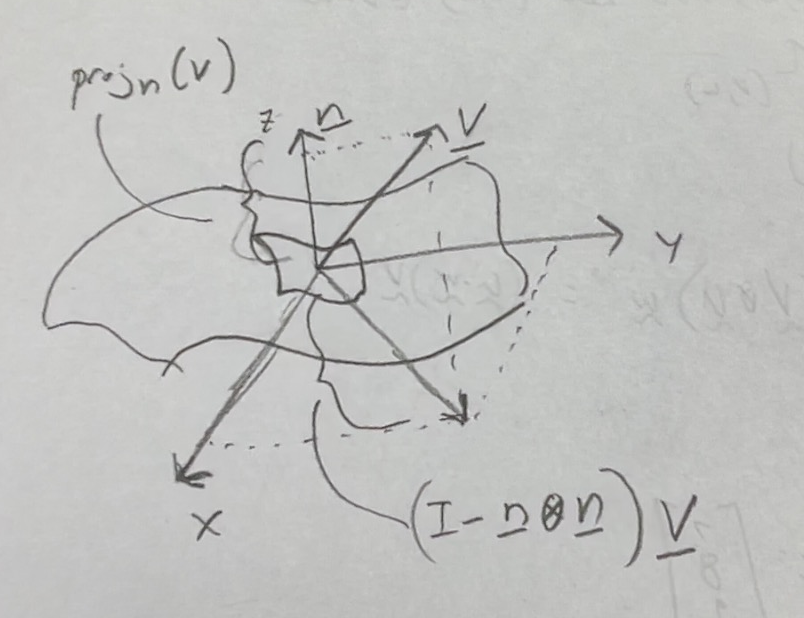
\includegraphics[width=.5\textwidth]{Figures/p2b.png}
    \caption{}
    \label{fig}
\end{figure}
\pagebreak
        \begin{problem}
            c) Let \(e\) and \textbf{f} be orthogonal unit vectors. Describe the geometric nature of the tensor \(e \otimes  e + \textbf{\textit{f}}   \otimes  \textbf{\textit{f}}  \)
        \end{problem}
        The geometric nature of \(e \otimes e + f \otimes f\) has the following effect upon vector \(\textbf{\textit{v}} \) :
\begin{align*}
    (e \otimes e + \textbf{\textit{f}}  \otimes \textbf{\textit{f}} )\textbf{\textit{v}} \\
    &=(e \otimes e)\textbf{\textit{v}} + (\textbf{\textit{f}} \otimes \textbf{\textit{f}} )\textbf{\textit{v}} \\
    &= (e \cdot \textbf{\textit{v}} )e + (\textbf{\textit{f}} \cdot \textbf{\textit{v}} )\textbf{\textit{f}} 
\end{align*}
This has the geometric interpretation of capturing the projections of a vector \(\textbf{\textit{v}} \)  in the direction of \(e\)  and \(\textbf{\textit{f}} \) , and removing the other components that the complete vector \(\textbf{\textit{v}} \)  may also contain.

        \begin{figure}[h]
    \centering
    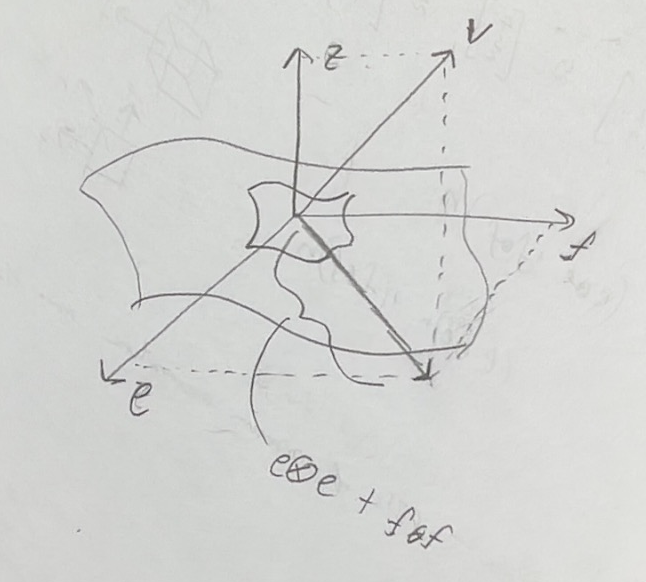
\includegraphics[width=0.5\textwidth]{Figures/p2c.png}
    \caption{}
    \label{fig}
\end{figure}

\end{document}
